\documentclass[a4paper, 12pt]{article}
\usepackage[utf8]{inputenc}
\usepackage{graphicx}
\usepackage{amsfonts}       % blackboard math symbols

\usepackage[portuges]{babel} % Traduz alguns campos de formatação para português

\setlength{\parindent}{1cm} % espaçamento do parágrafo
\usepackage{geometry} % configurar layout da página
\usepackage{setspace} % configurar o espaçamento de linhas
\usepackage{indentfirst} % alinhamento do texto, parágrafos

\usepackage{hyperref}

\usepackage{minted}

\newcommand{\inlineeqnum}{\refstepcounter{equation}~~\mbox{(\theequation)}} % Equação inliner junto com texto

\graphicspath{ {./images/} }

\usepackage{float} % tabela que nao fica fixa

\usepackage{siunitx}  % Package perfeita pra notacao cientifica
\RequirePackage{amsmath,amsthm,amssymb,hyperref} % Math 


\begin{document}
%\maketitle

\begin{titlepage}
	\begin{center}
	
	%\begin{figure}[!ht]
	%\centering
	%\includegraphics[width=2cm]{c:/ufba.jpg}
	%\end{figure}

		\Huge{Universidade Federal da Bahia}\\
		\large{Departamento de Engenharia Elétrica e Computacação - DEEC}\\ 
		\vspace{15pt}
        \vspace{95pt}
        \textbf{\LARGE{Relatório da Etapa I - Trabalho de Curto-Circuito - 2021.1  }}\\
		%\title{{\large{Título}}}
		\vspace{3,5cm}
	\end{center}
	
	\begin{flushleft}
		\begin{tabbing}
			Discentes: Henrique Nunes Poleselo, Leonardo Lima, Miguel Damásio\\

			Docente: Daniel Barbosa \\
	\end{tabbing}
 \end{flushleft}
	\vspace{1cm}
	
	\begin{center}
		\vspace{\fill}
			 Maio\\
		 2021
			\end{center}
\end{titlepage}
%%%%%%%%%%%%%%%%%%%%%%%%%%%%%%%%%%%%%%%%%%%%%%%%%%%%%%%%%%%

% % % % % % % % % % % % % % % % % % % % % % % % % %
\newpage
\tableofcontents
\thispagestyle{empty}

\newpage
\pagenumbering{arabic}


\section{Especificações}
Durante esta primeira etapa do trabalho de curto-circuito utilizou-se o software Anafas para validar os dados calculados pelos
scripts em Python que foram desenvolvidos. O sistema elétrico de potência que foi analisado em questão é mostrado na Figura \ref{fig:sep}. Sendo os requisitos para esta primeira etapa:

\begin{itemize}
    \itemsep0em 
    \item Diagrama de de sequência positiva;
    \item Matriz de impedância de base de sequência positiva;
    \item As tensões de pós-falta (\textit{Va}, \textit{Vb}, \textit{Vc}) em todas as barras em Volts e por unidade, nas suas respectivas referências, e as correntes, em Ampères e por unidade, nas linhas de transmissão (\textit{Ia}, \textit{Ib}, \textit{Ic}) circunvizinhas para os seguintes curtos-circuitos:
    \begin{itemize}
     \itemsep0em 
     \item Trifásico na barra da SE4 – 345kV com impedância de falta \\ $Z_f{_a} = 0,467 \si{\ohm}$
     \item Trifásico na barra da SE6 – 138kV com impedância de falta \\ $Z_f{_b} = 1,187 \si{\ohm}$
     \item Trifásico na barra da SE7 – 13,8kV com impedância de falta \\ $Z_f{_c} = 1,005 \si{\ohm}$
    \end{itemize}
\end{itemize}


\begin{figure}[h]
\centering
  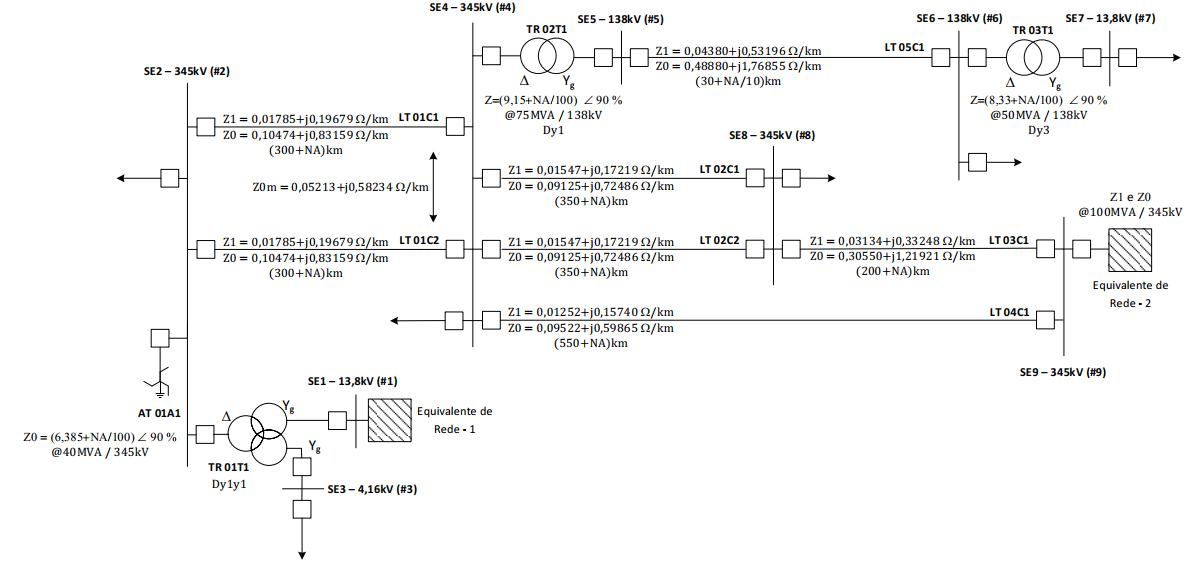
\includegraphics[scale=0.5]{img/Esquematic-ckt-geral.png}
\caption{Representação do SEP que foi analisado.}
\label{fig:sep}
\end{figure}

As tensões de pré-falta foram fornecidas:\\

\begin{table}[H]
\centering
\begin{tabular}{|c|c|c|c|}
    \hline
    Barra & Módulo(PU) & Angulo \\ \hline
    \num{1} & \num{1,0394} & \num{-13,8148}º  \\ \hline
    \num{2} & \num{1,0266} & \num{-13,8715}º  \\ \hline
    \num{3} & \num{1,0346} & \num{-14,0869}º  \\ \hline
    \num{4} & \num{1,0222} & \num{-13,6568}º  \\ \hline
    \num{5} & \num{1,0166} & \num{-20,6902}º  \\ \hline
    \num{6} & \num{1,0161} & \num{-21,1685}º  \\ \hline
    \num{7} & \num{0,9891} & \num{-26,0122}º  \\ \hline
    \num{8} & \num{1,0136} & \num{-12,2356}º  \\ \hline
    \num{9} & \num{1,0207} & \num{-8,8582}º  \\ \hline
\end{tabular}
\caption{Tabela das tensões de pré-falta.}
\end{table}

\section{Desenvolvimento dos Scripts}

O ponto de partida para o cálculo das tensões de pós-falta é primeiro determinar o diagrama de sequência positiva, também conhecido como a matriz ZBarra, que se encontra na Figura \ref{fig:zbarra} em anexo a este relatório, a mesma representa as relações de impedância existentes entre as barras do sistemas elétrico de potência. O script que realiza o cálculo referente ao ZBarra se encontra em anexo a este relatório, com o nome \textit{calc-zbarra.py}. É importante salientar que para a realização da etapa 1, a resolução foi dividida em dois diferentes programas, portanto é necessário rodar primeiramente o \textit{calc-zbarra.py}, que gerará um arquivo CSV com o \textit{zbarra.csv} que é importado no segundo programa \textit{calc-tensao-pos-falta.py}, que realiza o cálculo das correntes de falta, tensões pós-falta e correntes circunvizinhas. \\

O passo a passo para o cálculo da matriz ZBarra pode está descrito no respectivo código. Usou-se a impedância equivalente vista da barra $Z_1_{e_{_q}} = {0,05719$ com ângulo de $85,20976$º e a potência de curto circuito trifásico, $S_c{c_{_{3}}}$, ambos fornecidos nas tabelas de instrução do trabalho.  $S_c{c_{_{3}}}$ = 29761,6736\textit{W} com ângulo de 86,9873º. 
    
Para o cálculo das tensões de pós falta foi necessário inicialmente determinar as correntes de falta, visto que a variação das tensões nas barras é resultado da corrente de falta passante entre elas, logo da matriz de impedâncias tem-se que:

\begin{equation}
    V_p{_o_{s}} = V_p{_{ref}} + Z_k{_k} \cdot I_{f_{k}}
\end{equation}

Onde $V_p{_o_{s}}$ representa a tensão de pós-falta, $V_p{_{ref}}$ a tensão de pré-falta, $Z_k{_k}$ o elemento da matriz ZBarra (onde o k representa a barra em que a falta ocorre) e $I_{f_{k}}$ a corrente de falta. Para computar a tensão de pós-falta, é necessário primeiro calcular a corrente de falta. Tal corrente é calculada pela expressão (2) abaixo aplicada à barra onde ocorreu a falta:

\begin{equation}
    I_{f_{k}} = \frac{V_p{_{ref}}}{Z_{f_{k}} + Z_{t_h{_k}}}
\end{equation}

Lembrando que as tensões de pré-falta $V_p{_{ref}}$ constam na Tabela 1, já as resistências de falta $Z_{f_{k}}$ foram dadas também e são referenciadas tanto no script quanto neste relatório como sendo $Z_f{_a}$, $Z_f{_b}$ e $Z_f{_c}$, cada uma representando a resistência de falta nas barras 4, 6 e 7, respectivamente. O termo $Z_{t_h{_k}}$ é impedância de Thévenin vista da barra do curto, o mesmo pode ser obtido por meio do elemento $Z_k{_k}$ da matriz ZBarra, portanto, a equação é reescrita da forma:

\begin{equation}
        I_{f_{k}} = \frac{V_p{_{ref}}}{Z_{f_{k}} +Z_k{_k}}
\end{equation}

Por meio do script desenvolvido em Python, obteve-se a seguinte saída do programa, \textit{i.e}: as seguintes correntes de falta:

\begin{minted}[fontsize=\footnotesize]{objc}
Corrente de Falta na barra 4 é: Módulo(PU): 32,12584109102582 Fase(graus): -68,51850
Corrente de Falta na barra 4 é: Módulo(kA): 5,376192174448375 Fase(graus): -68,51850

Corrente de Falta na barra 6 é: Módulo(PU): 4,225277450856896 Fase(graus): -107,41853
Corrente de Falta na barra 6 é: Módulo(kA): 1,7677283142413658 Fase(graus): -107,41853

Corrente de Falta na barra 7 é: Módulo(PU): 1,466534145035217 Fase(graus): -153,21178
Corrente de Falta na barra 7 é: Módulo(kA): 6,135535387042465 Fase(graus): -153,21178
\end{minted}

Obtidas as correntes de falta relativas aos curtos nas respectivas barras e feitas as devidas defasagens em relação aos transformadores existentes no SEP é possivel obter as tensões de pós-falta em todas as barras do sistema, a tabela que contem as tensões pós-falta calculadas pode ser encontrada na Figura \ref{fig:posfalta}.
    
Para o cálculo das correntes circunvizinhas utiliza-se a Lei de Ohm, uma vez que estas são calculadas por meio da diferença entre as tensões de pós-falta presentes em barras adjacentes a barra do curto, divididas pelas impedâncias das linhas de transmissão ou pela reatância do transformador, a depender do caso. A tabela que contém os cálculos feitos no script pode ser encontrado na Figura \ref{fig:correntes}. O cálculo detalhado foi comentado devidamente no script \textit{calc-tensao-pos-falta.py}.

\section{Simulações}
\subsection{Determinação do Disjuntor 52-1 na Barra 4}
Para o dimensionamento do disjuntor 52-1, foi especificado que a tensão nominal do disjuntor é a tensão pré-falta na barra 4 e a corrente nominal do disjuntor será determinada pela corrente de curto. Sendo a barra 4 diretamente ao terra, sendo o este o pior caso. Conforme mostrado na Figura \ref{fig:item4}, os parâmetros comerciais devem ser de 380kV e 5kA.

\begin{figure}[h]
\centering
  \includegraphics[scale=0.4]{img/ITEM 4 - CORRENTE MÁXIMA DE CURTO NA BARRA 4.png}
\caption{Corrente máxima de curto na barra 4.}
\label{fig:item4}
\end{figure}

\subsection{Impedância do transformador TR03T1}
Através das simulações, uma falta trifásica na barra 7 sem impedância, observou-se que quando o transformador TR03T1 tem a sua reatância alterada para aproximadamente 28\% PU, a corrente de falta na barra 7 alcança o valor de aproximadamente 8kA, de forma que conforme ao diminuir esta porcentagem a corrente aumenta.
\begin{figure}[h]
\centering
  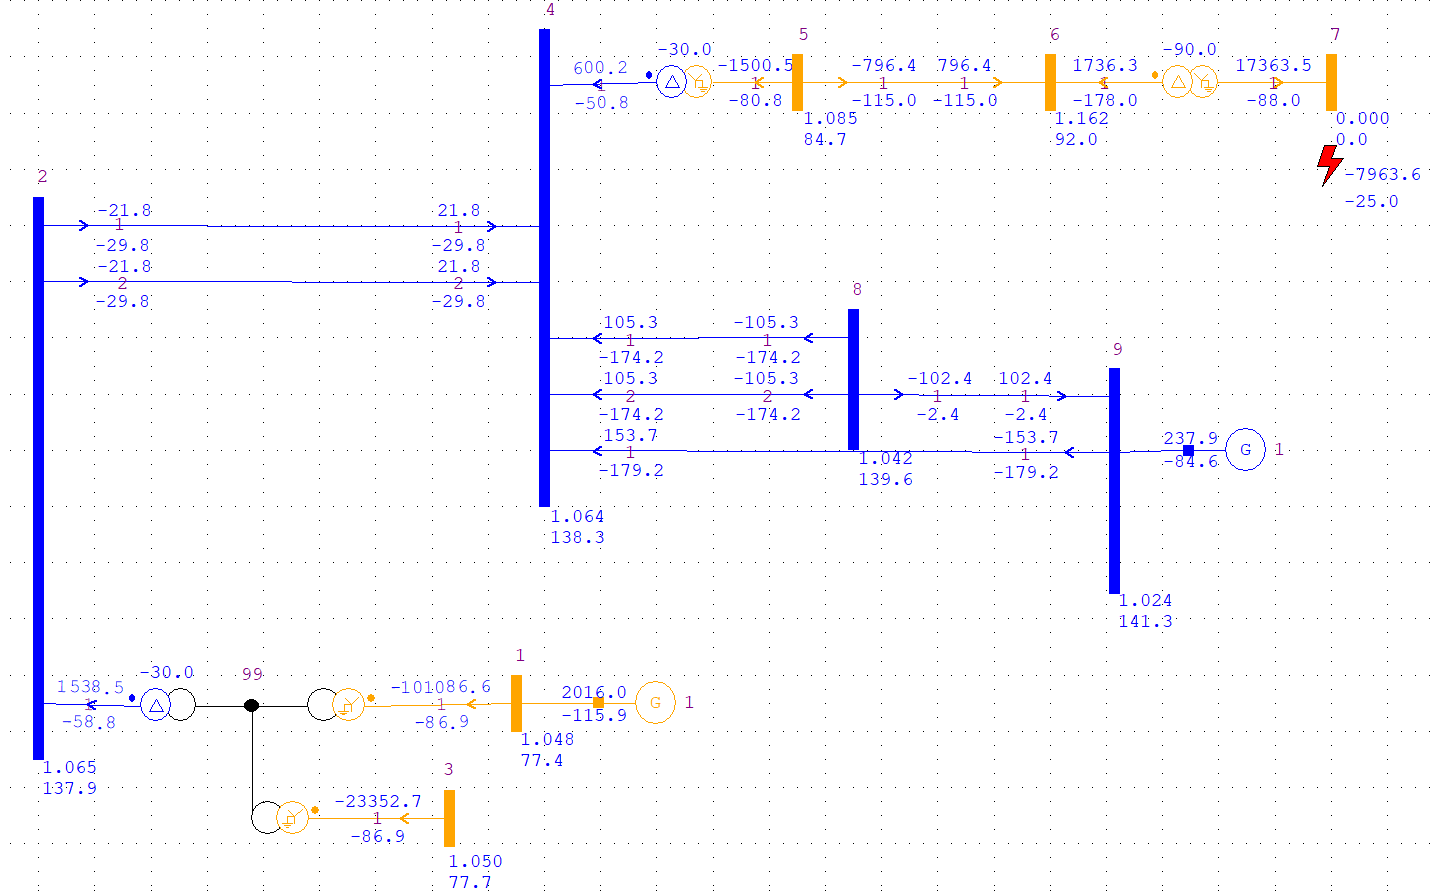
\includegraphics[scale=0.35]{img/ITEM_5_CORRENTE_DE_CURTO_NA_BARRA_7_SEM_IMPEDÃNCIA_E_REATÂNCIA_DO.png}
\caption{Simulação da falta trifásica na barra 7 sem impedância com o transformador em 28\% PU.}
\label{fig:item5}
\end{figure}


\subsection{Determinação da potência de curto-circuito na barra 8}
Primeiro passo foi determinar a capacidade de interrupção do disjuntor na barra 8 através da simulação do curto citcuio trifásico sem impedança na mesma, no caso 4.9kA, como mostrado na Figura \ref{fig:item6}.
\begin{figure}[h]
\centering
  \includegraphics[scale=0.35]{img/ITEM 6 - CORRENTE MÁXIMA DE CURTO NA BARRA 8.png}
\caption{Pior caso: máxima corrente de curto na barra 8.}
\label{fig:item6}
\end{figure}

Foi inserido o gerador na barra 8 e determinou-se a sua impedânca equivalente que é capaz de fazer com que a sua corrente de curto trifásico na barra 8 aumente em 20\%. Conforme as Figuras \ref{fig:item62} e \ref{fig:item63}, é possível perceber que esta impedância é de 0.5\% de resistência e e 17.5\%. A partir desta impedância foi determinado que a potência de curto-circuito trifásica é de 587MVA, atraveś da equação:

\begin{equation}
        S_c{c_{_{3}}} = \frac{V_p{_{ref}}^2}{conjZ_e{_q}}}
\end{equation}

\begin{figure}[h]
\centering
  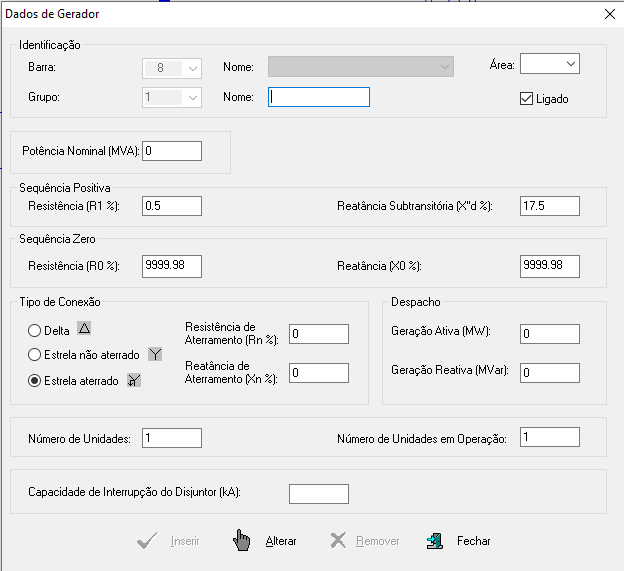
\includegraphics[scale=0.35]{img/ITEM 6 - DADOS DO TRAFO UTILIZADO.png}
\caption{Impedância do gerador utilizada para o cálculo da potência de curto-circuito máxima.}
\label{fig:item62}
\end{figure}

\begin{figure}[h]
\centering
  \includegraphics[scale=0.35]{img/ITEM_6_CORRENTE_MÁXIMA_DE_CURTO_NA_BARRA_8_COM_A_CARGA_INSTALADA.png}
\caption{Simulação de curto-circuito trifásico na barra 8 com o gerador inserido.}
\label{fig:item63}
\end{figure}

\subsection{Alteração da Configuração dos Transformadores}
A Figura \ref{fig:dy1} ilustra o circuito base com a falta trifásica com impedância na barra 7 com os transformadores configurados em Dy1. Já a Figura \ref{fig:yyo} com as mesmas configurações anteriores, só que com o transformador na configuração Yyo. Atraveś da simulação pode-se perceber que o módulo das tensões nas barras permanecem inalterados, já que este não depende da configuração dos transformadores. Já o ângulo das tensões pós-falta nas barras é alterado, uma vez que o grupo vetorial dos transformadores foi alterado, alterando-se assim os defasamentos entre barras. 

\begin{figure}[h]
\centering
  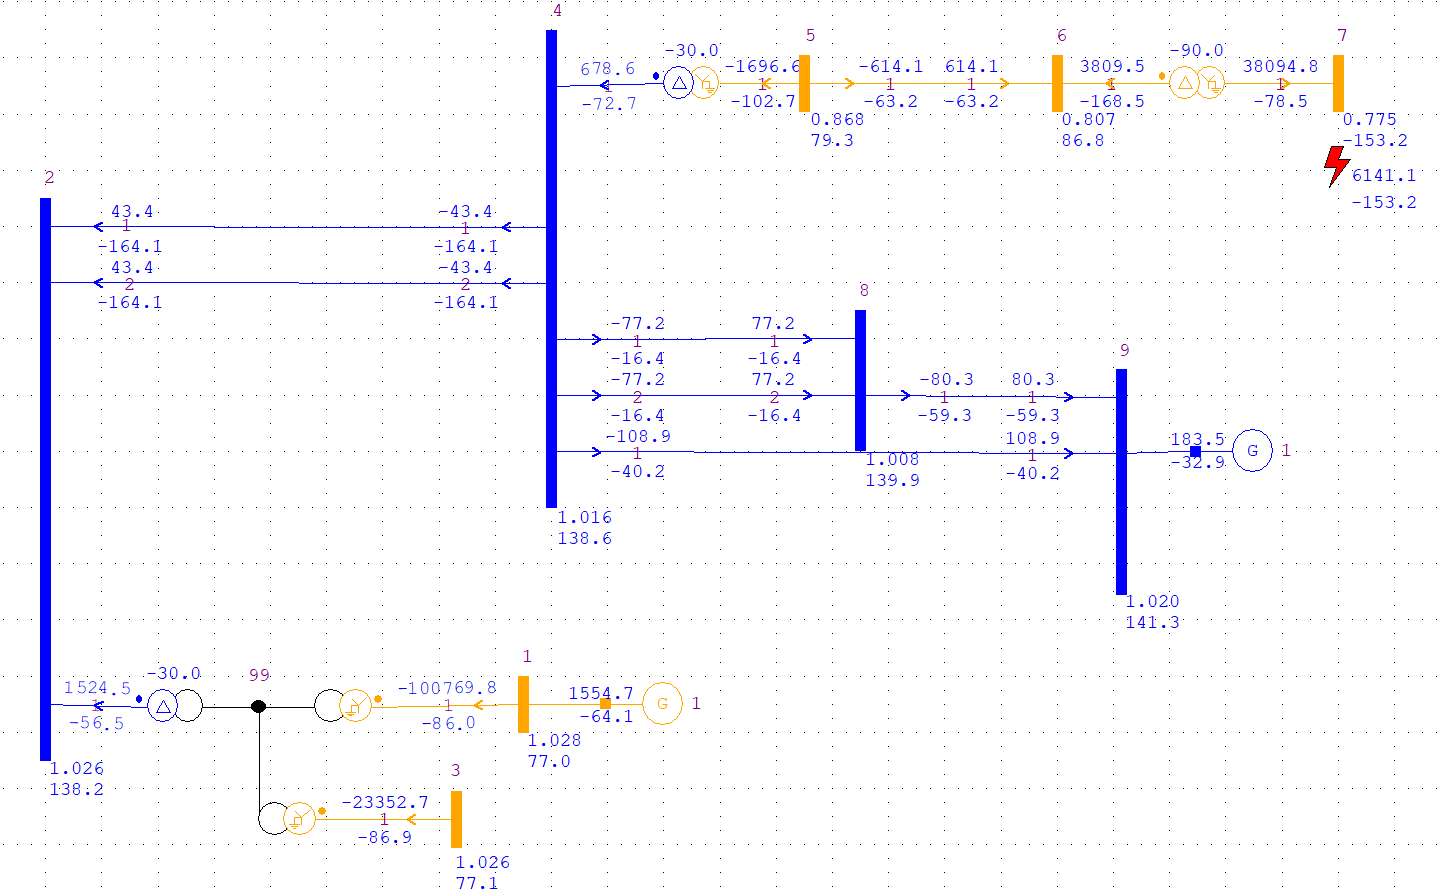
\includegraphics[scale=0.35]{img/ITEM 7 - CIRCUITO COM A FALTA NA BARRA 7 E TRAFO Dy1.png}
\caption{Transformador com configuração Dy1.}
\label{fig:dy1}
\end{figure}

\begin{figure}[h]
\centering
  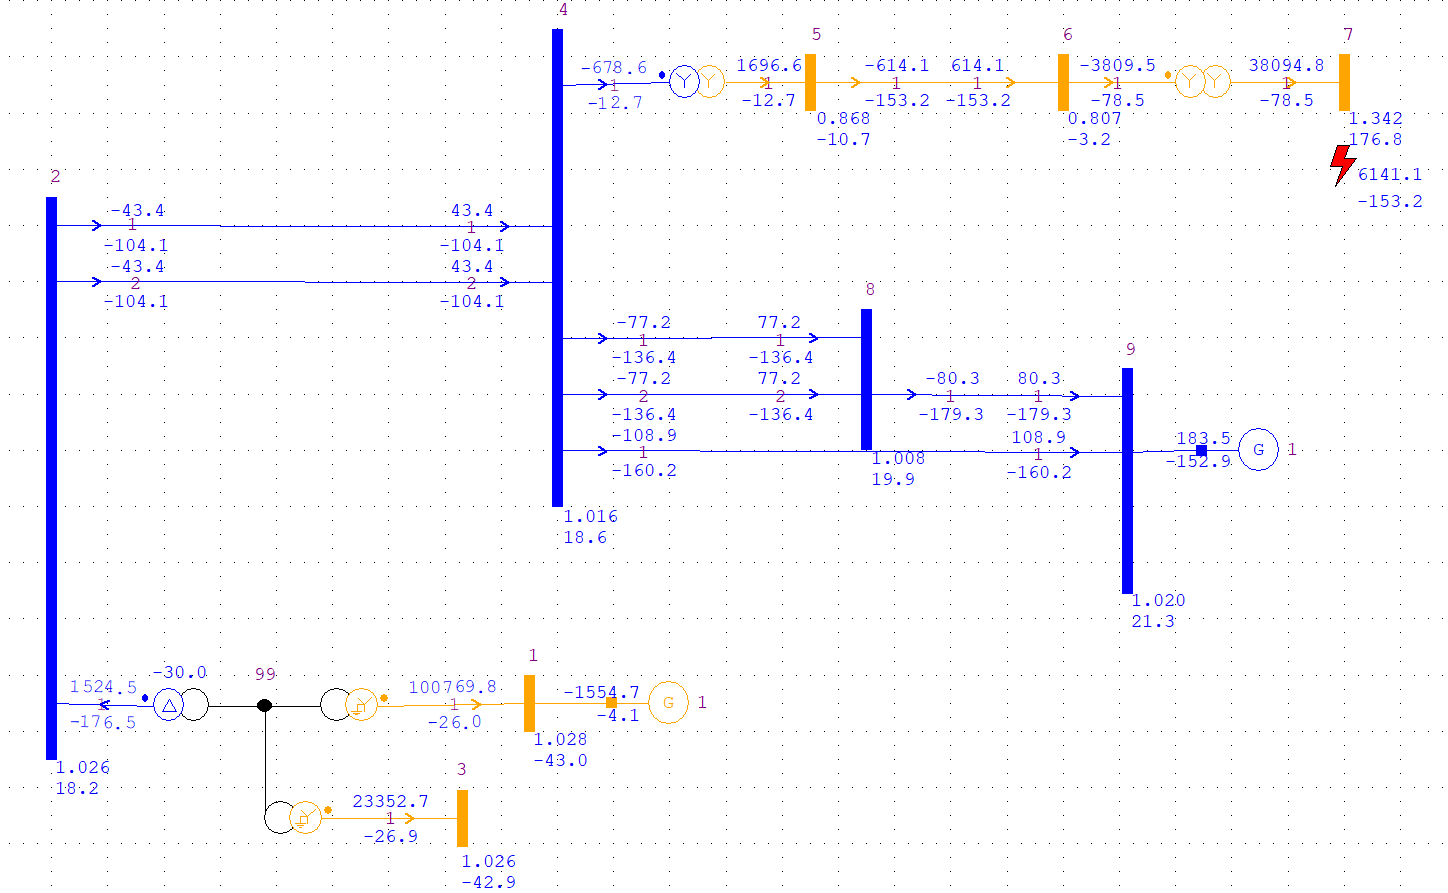
\includegraphics[scale=0.35]{img/ITEM 7 - CIRCUITO COM A FALTA NA BARRA 7 E TRAFO Yyo.png}
\caption{Transformador com configuração Yyo.}
\label{fig:yyo}
\end{figure}





\newpage
\addcontentsline{toc}{section}{Anexo}
\begin{figure}[h]
\centering
  \includegraphics[scale=0.37]{img/YBarra.png}
\caption{YBarra e ZBarra.}
\label{fig:zbarra}
\end{figure}


\begin{figure}[h]
\centering
  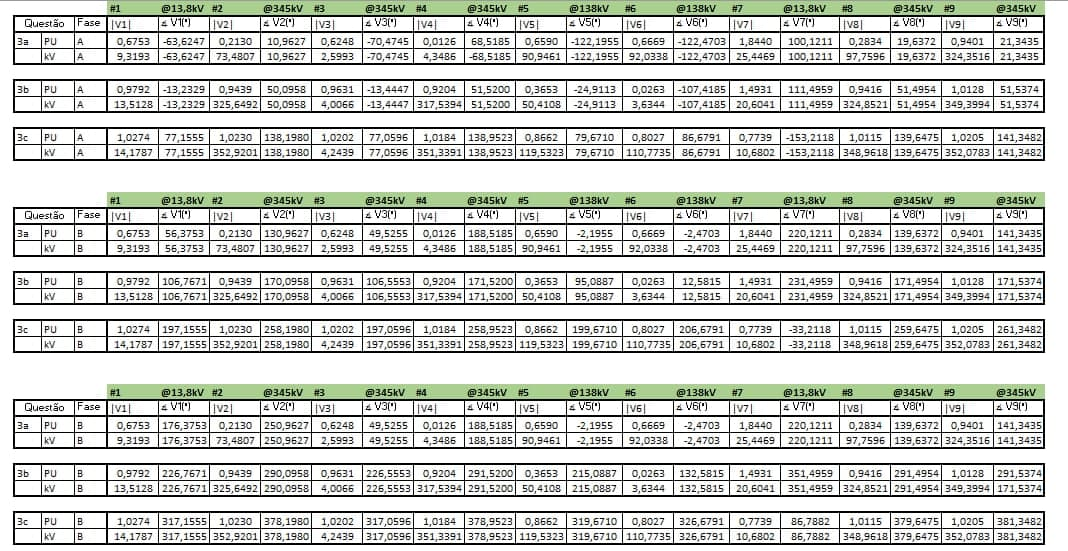
\includegraphics[scale=0.6]{img/tensoes.jpg}
\caption{Tensões pós-falta.}
\label{fig:posfalta}
\end{figure}

\begin{figure}[h]
\centering
  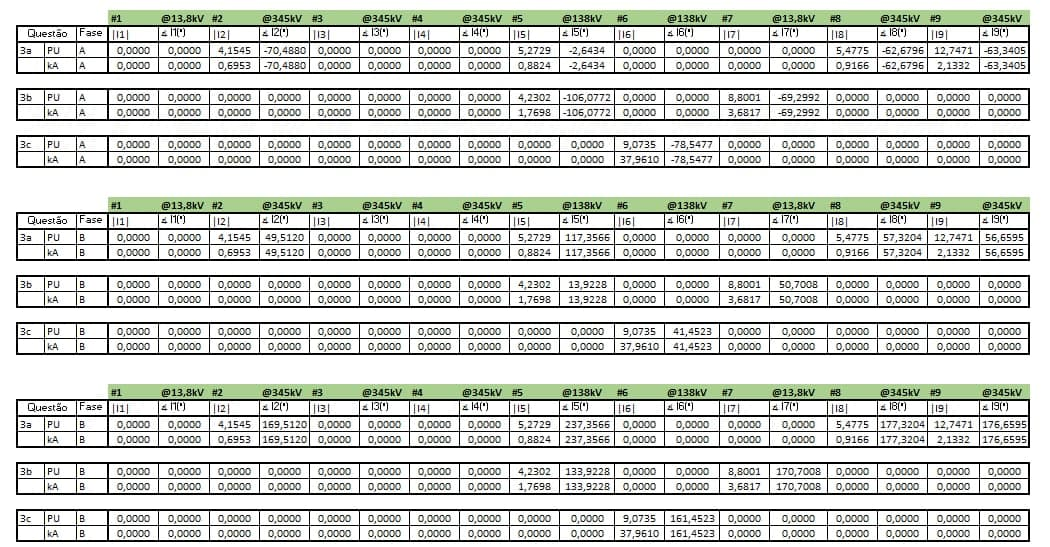
\includegraphics[scale=0.6]{img/correntes.jpg}
\caption{Tabela ilustrando as correntes que fluem de determinada barra para a barra onde ocorre a falta.}
\label{fig:correntes}
\end{figure}

\end{document}